\section{Title}

\subsection{Modelling}

x

The modelling of the system in a virtual environment is an important step to
allow experiments to be done in a simulator. The simulated experiments can be
replicated and repeated more easily, providing more data to analysis of the
applied algorithms. Also, most algorithms used in autonomous robotic navigation
is dependant on fine tuned parameters to fit the needs of the application in case.
With simulations these parameters and its effects can be better understood and
be set more closely to the desired ones in the real scenario.

With this concern with parametrization and experiment replicability in mind the
CaRINA platform was modelled to be simulated in Gazebo, a physics simulator
provided in ROS environment.  \ldots \ldots

There are othes 3D simulatos that is somehow integrated with ROS, but Gazebo is
more tightly closed and is designed with ROS in mind, so, is the native choice
when working with ROS. Actually, its physics simulation is based on ODE and 
provides only ridgid body dynamics, but others physical simularion libraries
like Bullet and Simbody are being integrated.

Since our main purpose is to check and avoid collisions the current physical
simulation available in Gazebo is suitable for our robotics simulations.

---

The simulation environment give the ability to more researches at the same time
to test the platform and conduct experiments of each system component. The
results can be more easily exchanged and agregated by teams. 


This make quicker solutions developments 


\subsection{Another subtitle}

URDF is a language in XML formatting that is used basically to describe the
transform relations between the robot coordinates frames. Each moving part of
the robot and each sensor has its own reference coordinate frame for the
generated data. In ROS, all coordinate systems are kept by a component called
TF that is responsible to provide the transformed coordinate from one frame to
another. \ldots

Since these transforms must be done also in inverse order, the robot coordinates
frames are represented in a tree in a parent-child manner. By the other hand,
this tree obligates the representations of the robot in the URDF file to be
limited. Most physical simulation libraries uses the concept of links and joints
to describe physical relations of the structures of a body. A joint describe
a relation between links and both can present physical properties like friction
coefficients and elasticity. The links and joints are more suited to be
represented in a graph and this is way URDF can be limiting. 

The Gazebo simulatior is not limited by the URDF description format and more
complex physical relations can be represented, but, ROS still enforces the robot
to be represented in a tree like coordinate frames structure. 

Fortunatelly, URDF
can be extended with Gazebo specific notations to acomodate both
representations.

The CaRINA platform is targeted to car-like robots with the aim of autonomous
navigation of terrestrial vehicles. The project actually counts with two
platforms, one more suited for off-road scenarios and another for urban roads.
The modelling of both platforms don't differ much in simulation except for some
parameters.

When preparing the simulation environment we have two main concerns, the
realism of the scenarios and the car modelling. Since there is no much moving
parts in a car-like robot and the degrees of freedom are very restricted the
model itself can be well represented in the URDF tree format. 

The only mechanical structure that cannot be modeled and constrained directly by
URDF is the Ackermann steering arrangement that makes a loop with links and
joints, but with Gazebo extensions this can be done.



---

Gazebo allows to create component models that can be used to build a
simulated scenario. These models are described also by a XML language and can
contain 3D meshes for complex visual objects. 


For vision based solutions, the 3D scenario can be rendered to images with
virtual cameras, that can be adjusted with the desired poses and FOV. Stereo and
panoramic cameras can be simulated and used as sources for vision algorithms.

Gazebo also allows to simulate range sensors like lasers by raycasting on 3D
objects on the scene and generating the points measurements also with the
reflectivity intensities that can be parametrized in the objects color
materials.


\subsection{Another subtitle}


We use two main simulation scenarios that can be adapted for specific test
situations. First model is an unstructured scenario with an irregular terrain an
with some vegetations. One use of this kind of simulation are related to
agricultural sites where autonomous vehicles usage are being researched by our
group. In that scenario, vision based solutions has been the main focus. (and
the simulated environment ca)

The other kind of scenario is the urban ones, where 



===


We also put on the virtual model a suspension mechanism independant on each
wheel. Since our intentions are not to simulate the mechanical behaviour of the
car itself but our autonomous navigation systems, the suspension is an
aproximation model just enought to enable us to simulate on uneven terrains
avoiding the kicking collision effect with the ground caused by the ridgid body
physics simulation and keeping the four wheels in contact with the ground to
avoid loss of traction, splipages and unstable poses of the vehicle that
(wouldn't happen on the real case) diverges from real situations.

One other effect desired from the simulated suspension is the balancing of the
vehicle when bending, accelareting and breaking, that will have a direct effect
on the sensors reading and be more close to real situations. This give us a
better simulated IMU data with a more realistic associated noise.




%The others effects desired from the simulated suspension are some stabilization
%of simulated sensors readings like virtual images 






 %************************************************************************************************************************
 \section{Platform}\label{sec:Plataform}
 
 In this work we used a 3D simulation model (Fig. \ref{fig:carina3D}) of the robotic platform called 
 CaRINA, 
 and also the real platform which is an electric vehicle adapted with sensors and actuators (Fig. \ref{fig:carinaReal}). 
 
 The perception system of the vehicle is composed by lidars, cameras, GPS, IMU and encoders. 
 Several combinations of these sensors may be mounted on the vehicle, making possible to develop work on areas of mobile robotics, 
 such as, localization, mapping, and motion planning. The vehicle also has actuators for steering and acceleration.
 % and more details of this platform may be found in \cite{Fernandes2012}.      
 
 
 \begin{figure}[!h]
     \centering
     \subfigure[3D Model]{\label{fig:carina3D}
         \includegraphics[width=0.195\textwidth]{figuras/carina3d.jpg}}        
     \subfigure[Vehicle]{\label{fig:carinaReal}
         \includegraphics[width=0.17\textwidth]{figuras/carina1.jpg}}
     \caption{Robotic Platform CaRINA}
 \label{fig:carina}
 \end{figure}
 
 
 The kinematic model of the vehicle is based on the Ackerman steering geometry represented by Fig.  
 \ref{fig:ackerman} \citep{pepy2008}. The front wheels are steered while the direction of the back wheels remains fixed. 
 The vehicle's pose with respect to an inertial coordinate system is represented by  $[x,y,\theta]^T$,  where $(x,y)$ is 
 the coordinate of a point in the middle of the axle of the back wheels, and $\theta$ is the vehicle's orientation. 
 The curvature radius of the vehicle is given by $\rho =\frac{L}{\tan{\delta}}$, where $\delta$ is the steering angle of the 
 front wheels, $L$ is the distance between axles, and $v$ is the linear velocity of the vehicle.
 
 \begin{figure}[!h]
 \centering
 \includegraphics[scale=0.24]{figuras/model_kinematic.png}
 \caption{Vehicle geometry representation.}\label{fig:ackerman}
 \end{figure}
 
 The kinematic model equations are given by 
   
 \begin{eqnarray}
     \left\{
         \begin{array}{ccc}
             \dot{x} = v \cos \theta 
             \\
             \dot{y} = v \sin \theta 
             \\
             \dot{\theta} =  \frac{v}{L}\tan \delta
         \end{array}
     \right.
 \label{eq1}
 \end{eqnarray}
 
 The 3D model was created for the Gazebo simulation environment \citep{Gazebo}  based on the real vehicle, 
 considering its physical properties, the Ackerman kinematic model, and the embeded sensors. In this work, 
 three LIDARS have been used for obstacle detection. They were positioned on the vehicle in such a way that it is 
 possible to detect obstacles $360^o$ around it.
 

 
 
 
 ====
 
 
\begin{figure}[ht]
	\begin{minipage}[b]{1\linewidth}
	    \centering
	    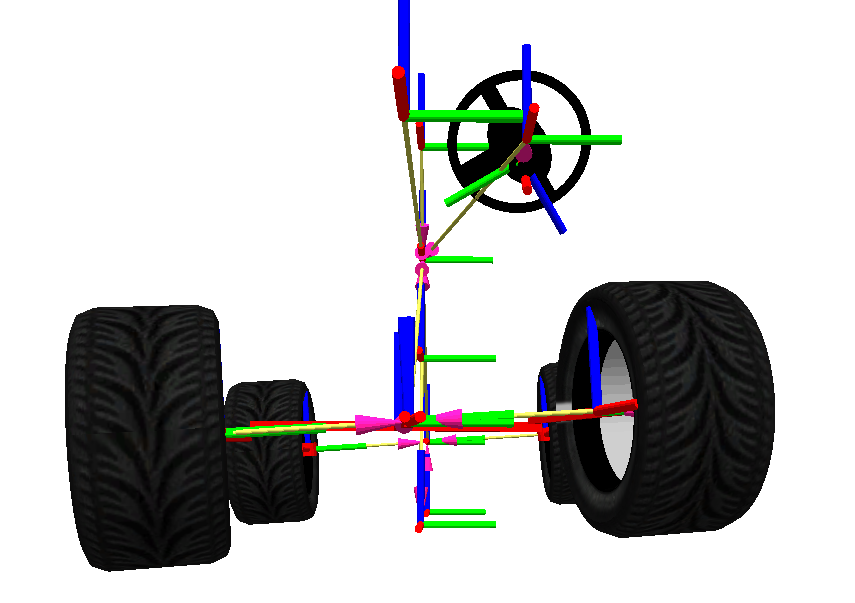
\includegraphics[width=\textwidth]{modelo_carina/carina_rviz_uneven_susp.png}
	 	\caption{Suspension effect on an uneven terrain}
	 	\label{fig:uneven}
	\end{minipage}
\end{figure}


\begin{figure}[ht]
	\begin{minipage}[b]{1\linewidth}
	    \centering
	    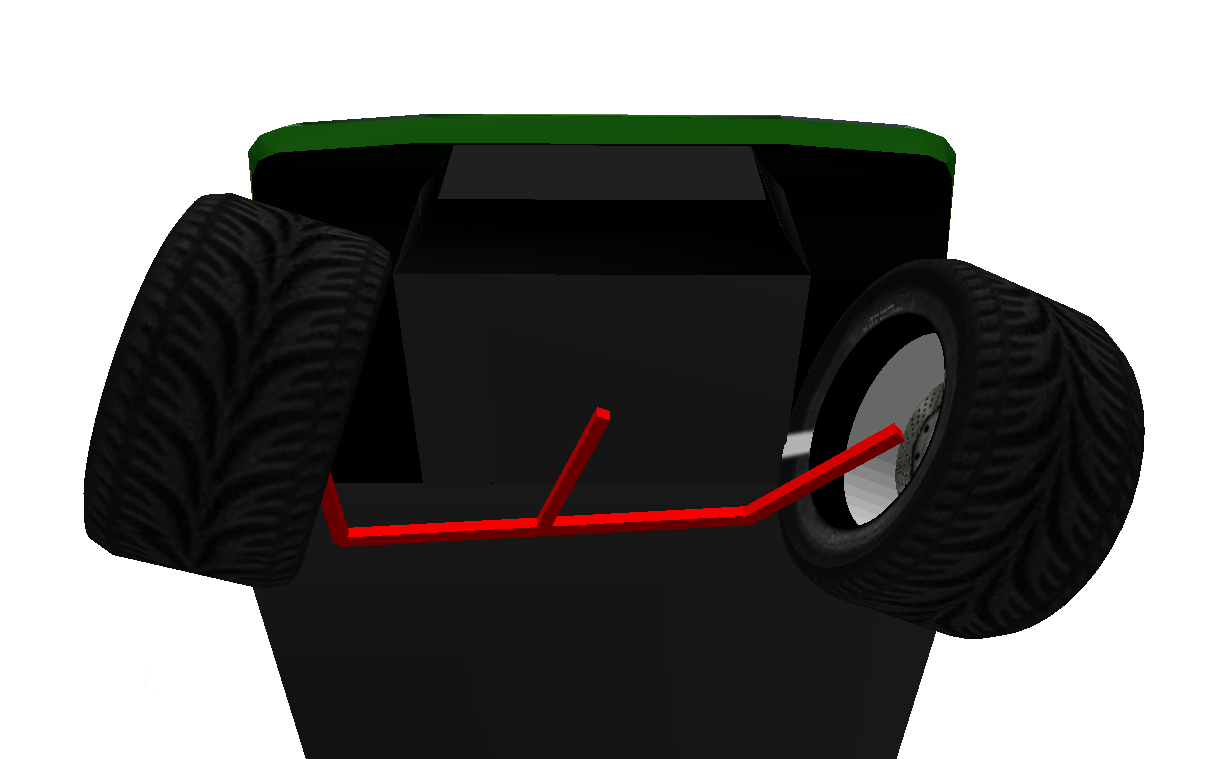
\includegraphics[width=\textwidth]{modelo_carina/carina_rviz_steering.png}
	 	\caption{Ackerman steering geometry modelled in simulation}
	 	\label{fig:ackermann}
	\end{minipage}
\end{figure}


\begin{figure}[ht]
	\begin{minipage}[b]{1\linewidth}
	    \centering
	    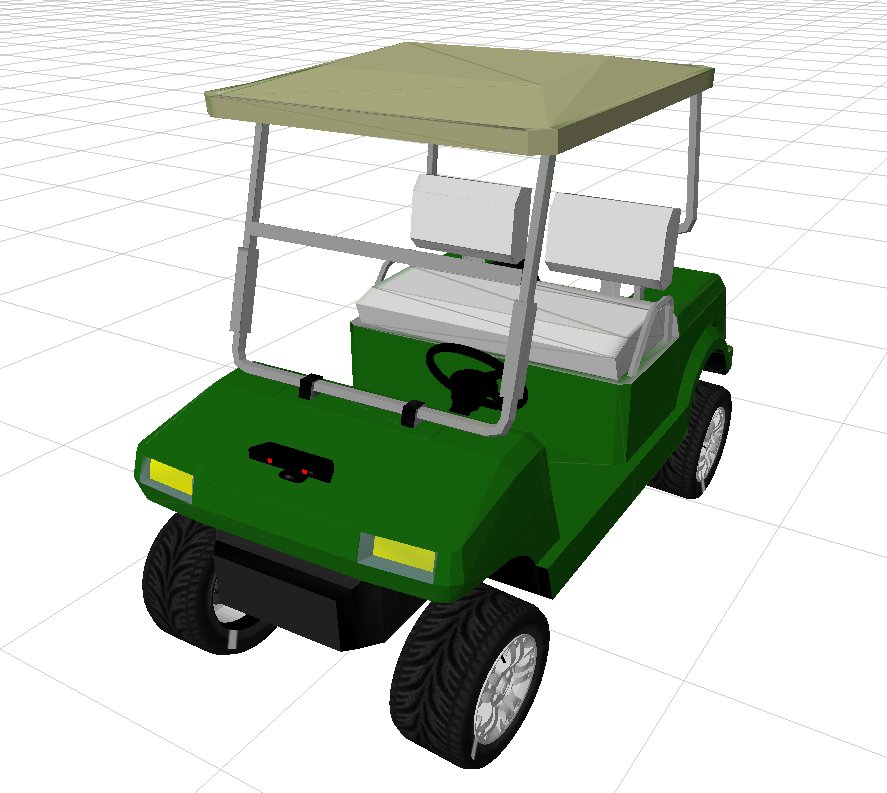
\includegraphics[width=\textwidth]{modelo_carina/carina_rviz_fundo_branco.png}
	 	\caption{CaRINA I virtual model}
	 	\label{fig:model}
	\end{minipage}
\end{figure}

\begin{figure}[ht]
	\begin{minipage}[b]{1\linewidth}
	    \centering
	    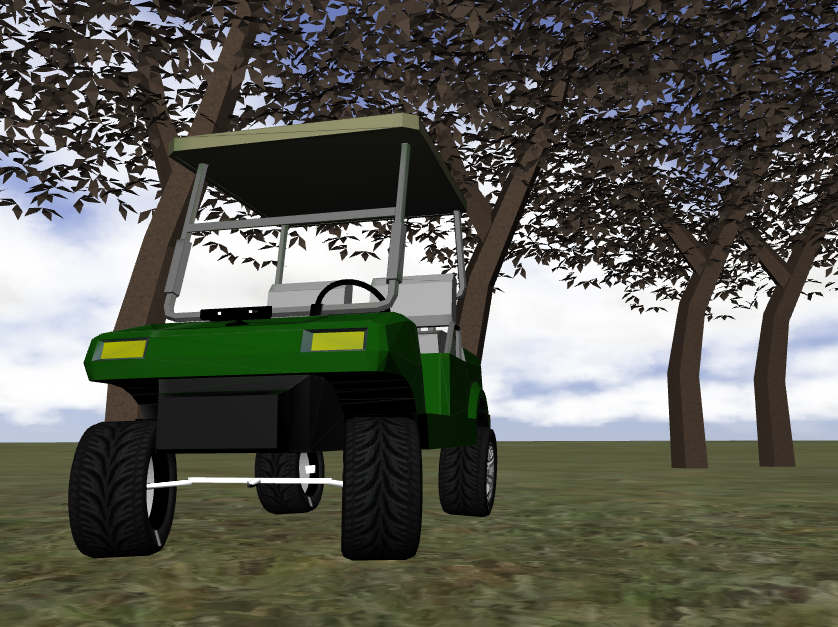
\includegraphics[width=\textwidth]{modelo_carina/carina_gazebo_frente_fundo.png}
	 	\caption{CaRINA I model on unstructured scenario in Gazebo simulator}
	 	\label{fig:gazebo}
	\end{minipage}
\end{figure}

\begin{figure}[ht]
	\begin{minipage}[b]{1\linewidth}
	    \centering
	    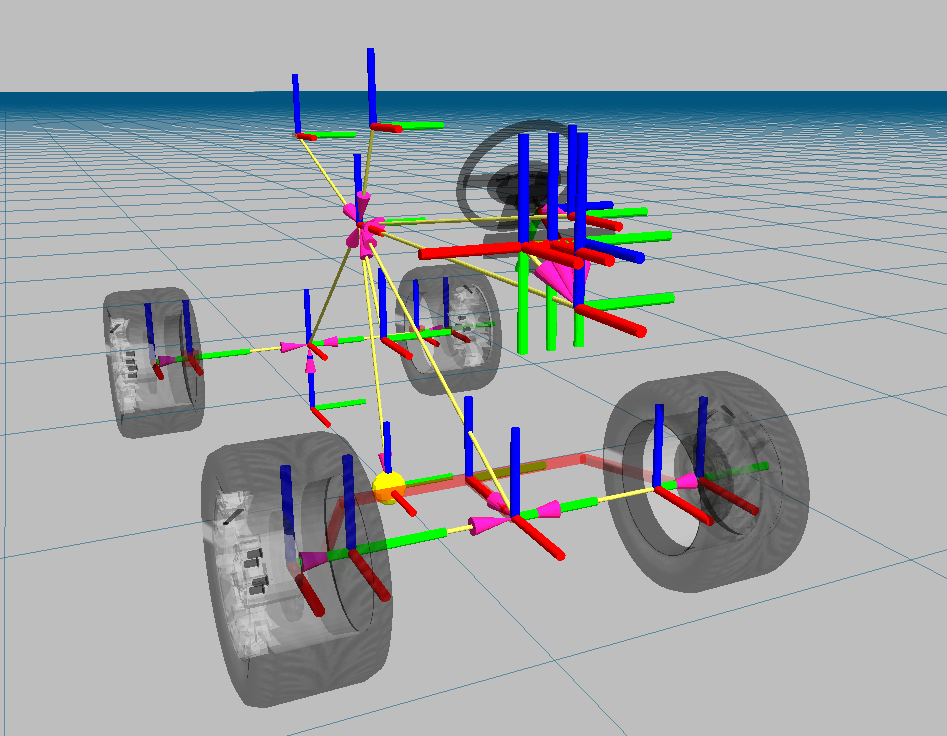
\includegraphics[width=\textwidth]{modelo_carina/carina_tf_wheels_transp.png}
	 	\caption{Transform frames (TF) reference cooridnates}
	 	\label{fig:tf}
	\end{minipage}
\end{figure}




